\section{RESULTS}\label{sec:reslts}
The system successfully ran generating valid trajectories.  The commanded trajectory produces the desired velocity of 4.9m/s.  The joint position of the physical joints were logged during runtime.  The logged and commanded trajectories are seen plotted over the SRM in Fig.~\ref{fig:svmMap}.  The velocity and acceleration of the end-effector for the logged and commanded trajectories in the velocity phase can be seen Fig~\ref{fig:posPlot}.  The end effector had large accelerations present when run on the physical system.  

\begin{figure}[thpb]
  \centering
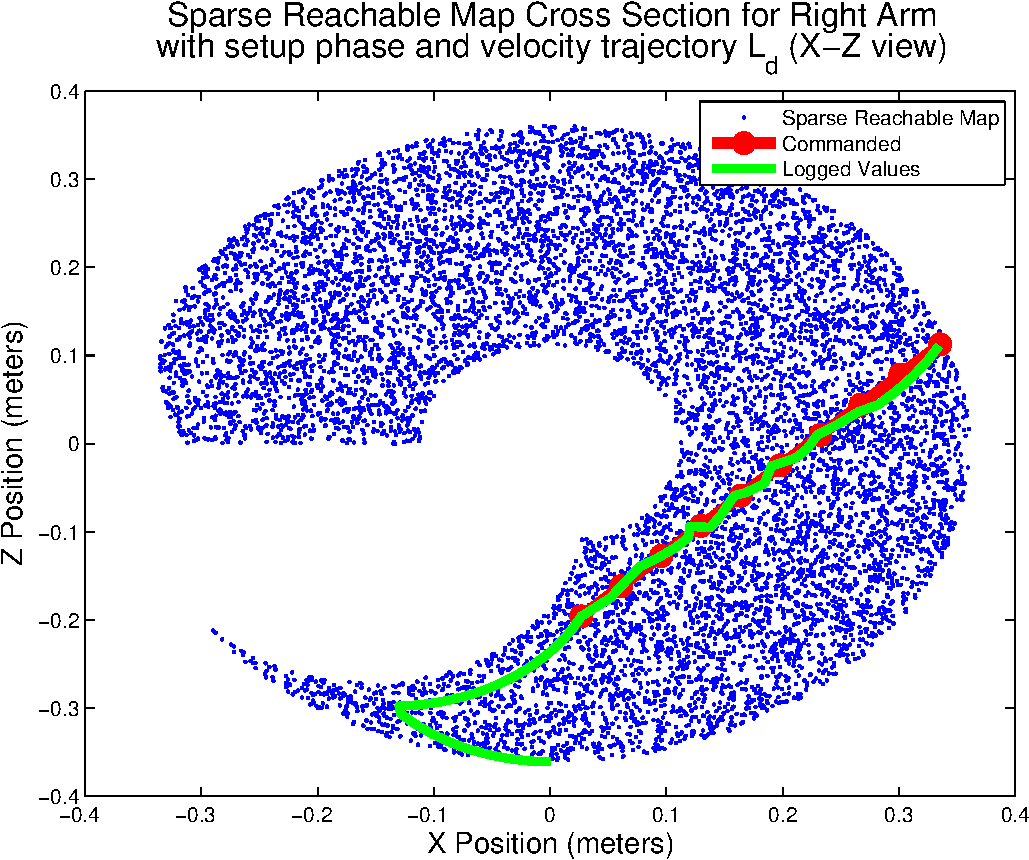
\includegraphics[width=1.0\columnwidth]{./MATLAB/throwTrajAct.pdf}
  \caption{Commanded right arm end-effector position in $R^3$ from Fig.~\ref{fig:3dThrowPlot1} (red) and the logged joint space values converted to $R^3$ using forward kinematics (green) shown over the sparse reachable map (blue).}
  \label{fig:svmMap}
\end{figure}

\begin{figure}[thpb]
  \centering
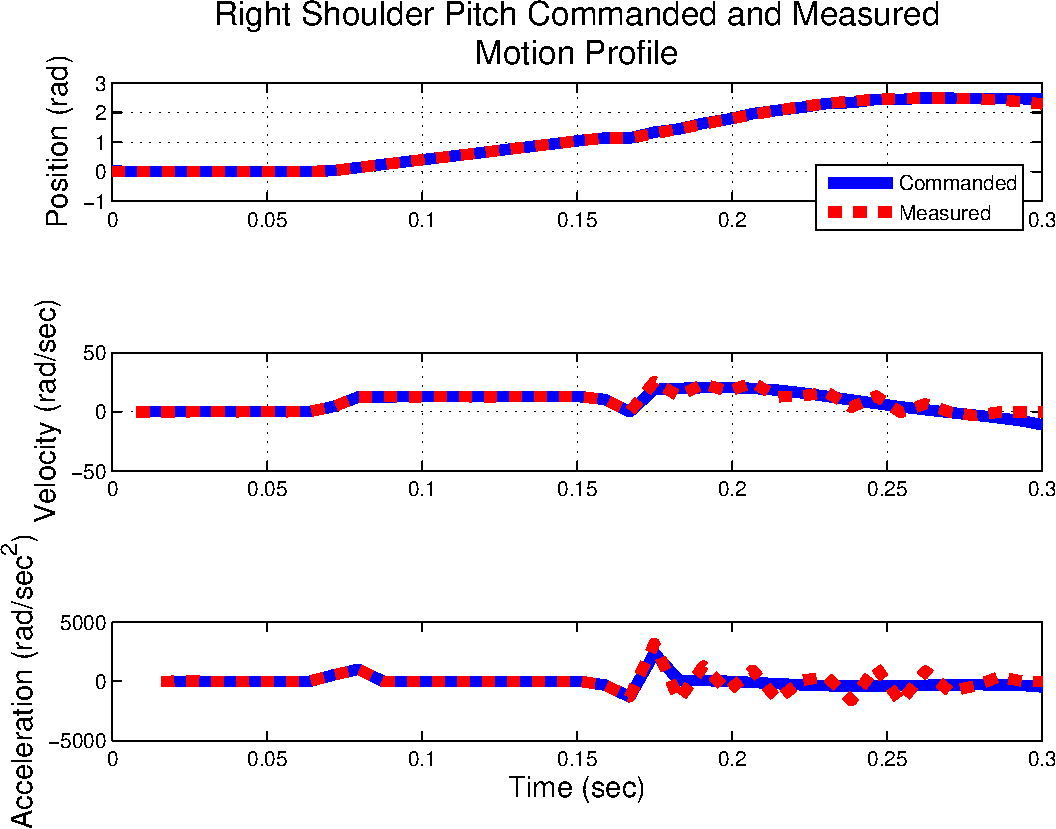
\includegraphics[width=1.0\columnwidth]{./MATLAB/throwTrajRSPplot.pdf}
  \caption{Right shoulder pitch commanded and measured motion profile; Position (top), Velocity (middle), Acceleration (bottom).  This is the result of running the trajectory shown in Fig.~\ref{fig:fThrow} and Fig.~\ref{fig:3dThrowReal}}
  \label{fig:velosPlot}
\end{figure}


The end effector has large accelerations present because some of the actuators are commanded with accelerations and torques beyond the capabilities of the physical actuator.  The angular velocity and acceleration of the right shoulder pitch joint can be seen in Fig.~\ref{fig:velosPlot}.  The large accelerations combined with the inertia of the arm caused the joint to overshoot the commanded position.  This caused over torque on the pitch joint causing the joint to shutdown in slightly less then 10\% of the trials.



\begin{figure}[thpb]
  \centering
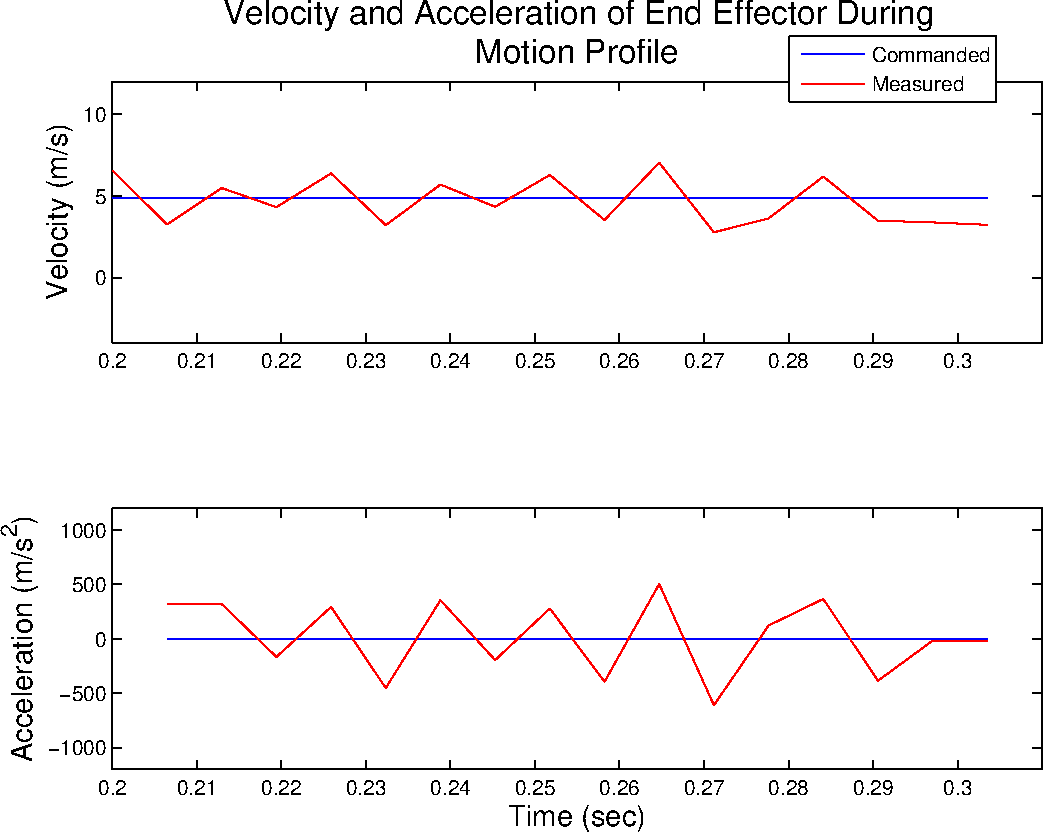
\includegraphics[width=1.0\columnwidth]{./MATLAB/throwTrajRSPacc.pdf}
  \caption{The velocity and acceleration of the end-effector for the commanded trajectory and the recorded runtime log in the velocity phase; Velocity (top), Acceleration (bottom).  The is the result of running the trajectory shown in Fig.~\ref{fig:fThrow} and Fig.~\ref{fig:3dThrowReal}.}
  \label{fig:posPlot}
\end{figure}








